\newpage{\clearpage}
\chapter{ Desarrollo y ejecuci\'{o}n del proyecto} 
\section{Arquitectura del proyecto}
El medidor se planteó con base a una arquitectura combinada entre software y hardware, en donde las cargas que  se miden serán la entrada inicial del sistema. Dicha entrada pasa por un proceso de converison y analizis de datos; estos resultados se pueden visualizar de manera gráfica y númerica en una aplicación web.\\\\
\begin{figure}[H]
    \centering
    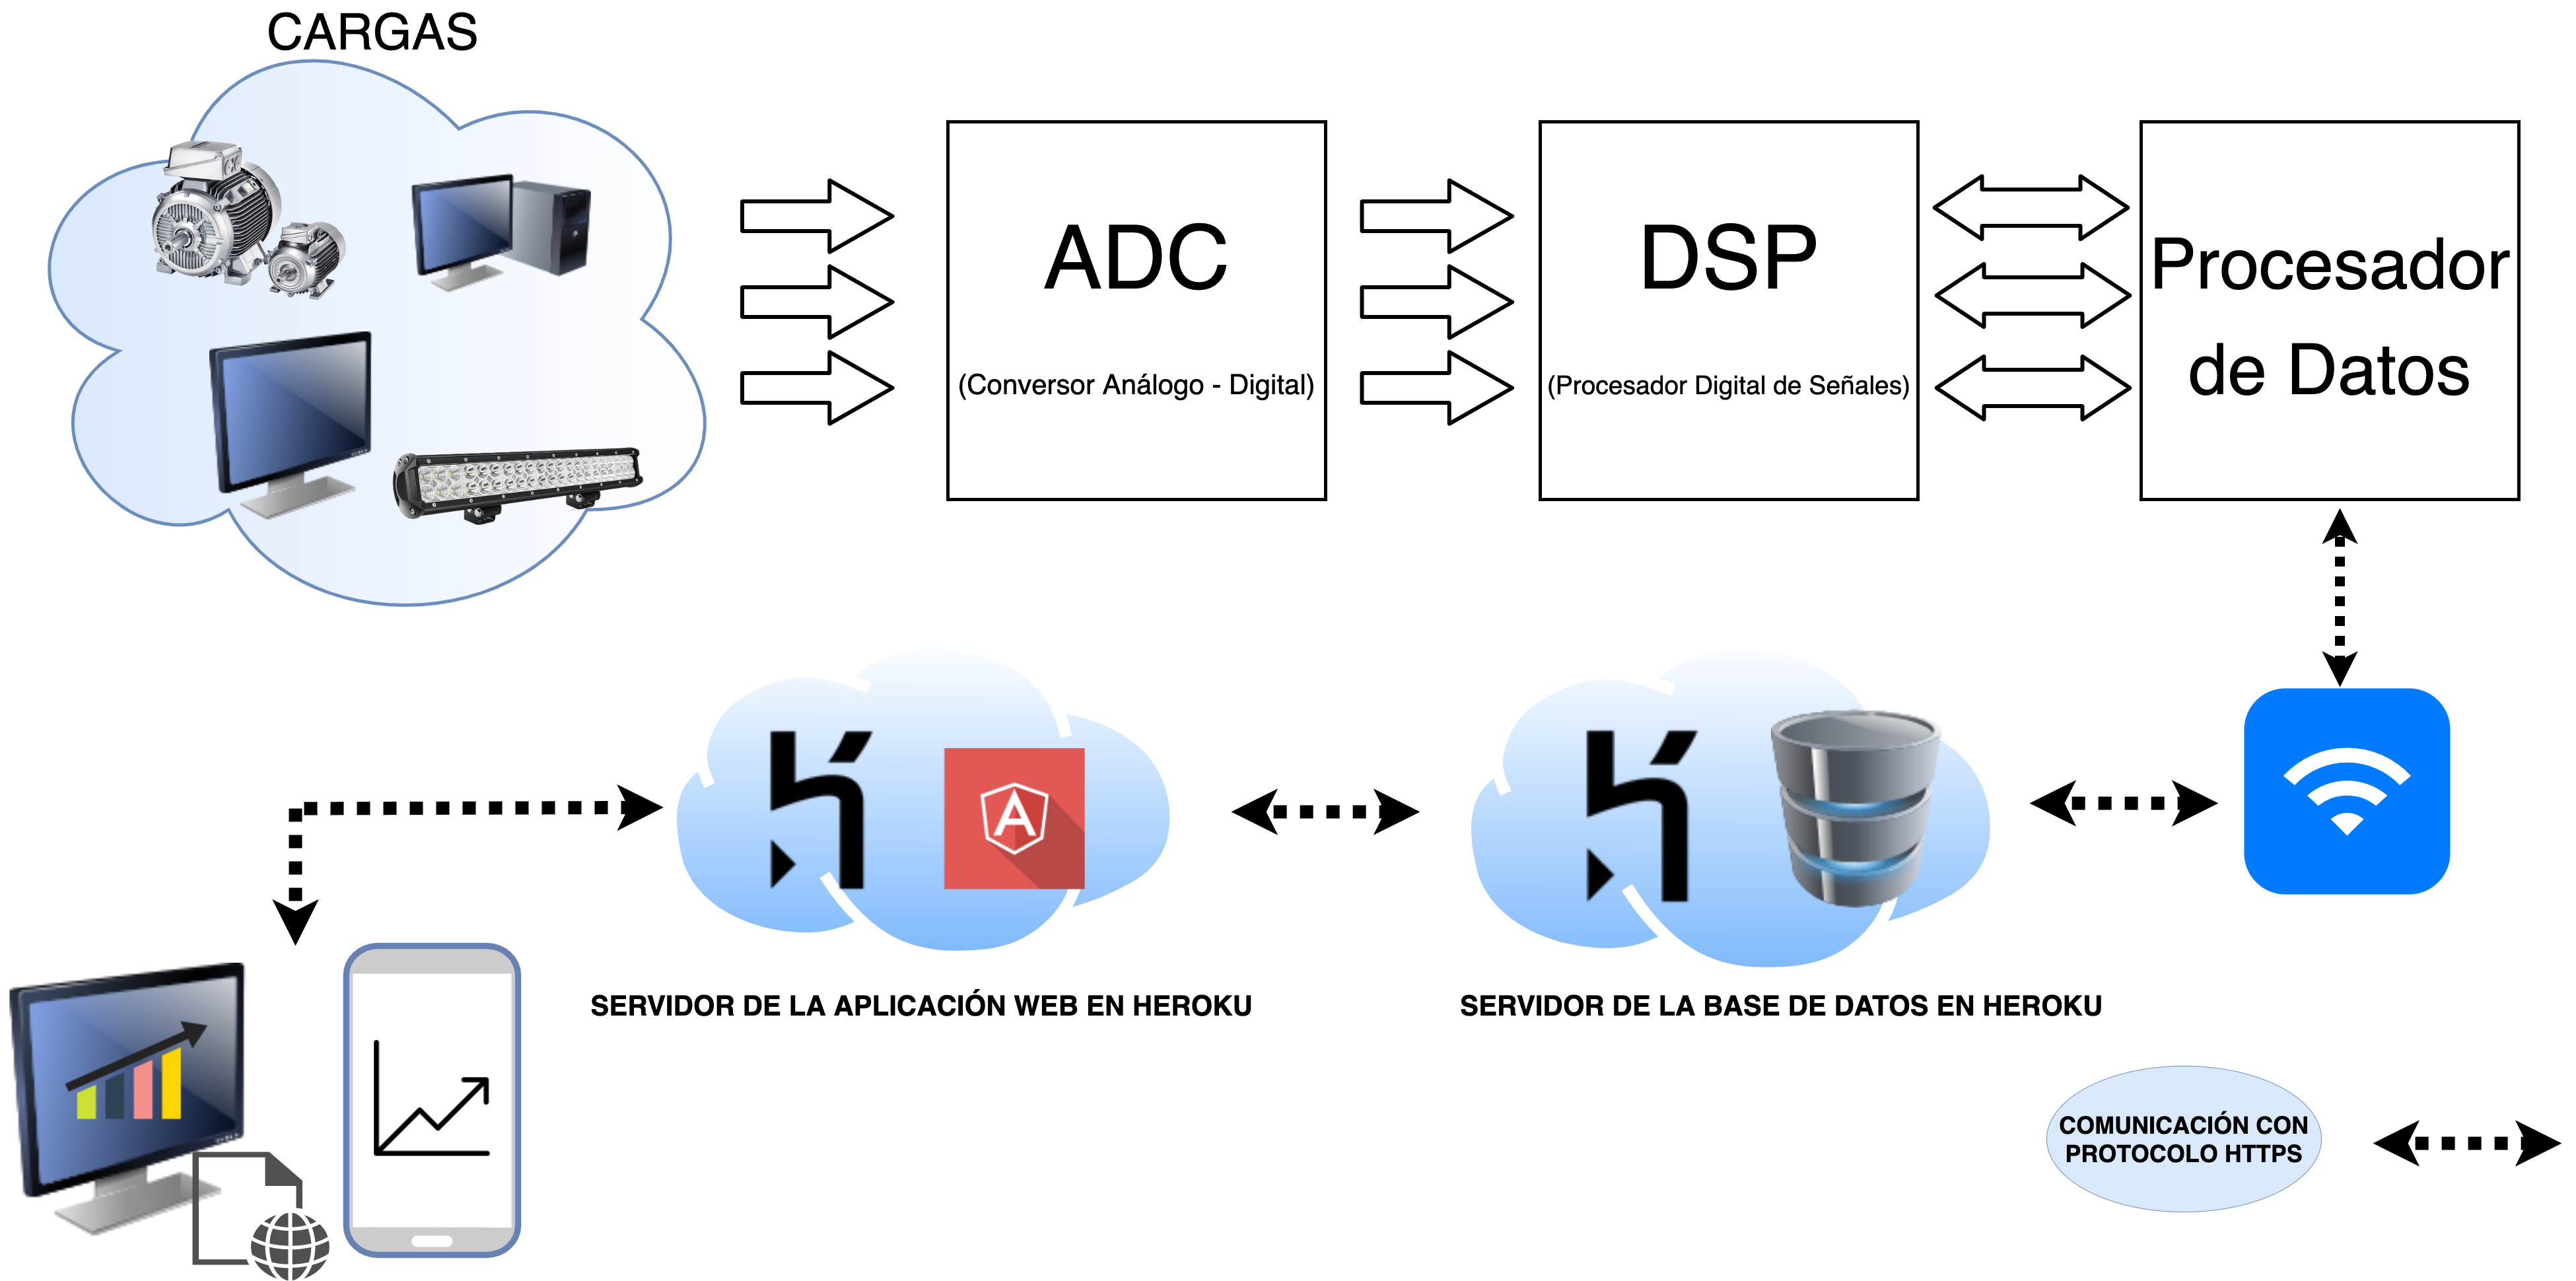
\includegraphics[width = 15cm]{3Proyecto/arquitectura}
    \caption{Arquitectura del proyecto} 
    \label{fig:arquitectura-proyecto}
    \end{figure}
El proceso de medición empieza en el momento de conectar una carga electrica al conversor de señal análoga a digital. Estas señales pasan a un procesador digital de señales, dónde se aplica los parámetros matemáticos establecidos en el estándar IEEE 1459 del 2010, el cual da la medición de la potencia eléctrica en cualquier tipo de condición.\\\\
% En primera instancia, se planteó el diseño electrónico del medidor, iniciando por las cargas donde se conectan a un conversor de señal análoga a digital, estas señales se pasan a un procesador digital de señales, dónde se aplica los parámetros matemáticos establecidos en el estándar IEEE 1459 del 2010, el cual da la medición de la potencia eléctrica en cualquier tipo de condición.\\\\
Dicho esto, la información se envía a un procesador de datos encargado de administrar la lectura, escritura y filtración de datos. El procesador debe contar con conexión a internet ya sea por via wifi o ethernet, con el fin de enviar la información al servidor de base datos alojado en la nube. La comunicación entre el procesador de datos y el servidor se realiza a través del protocolo de comunicación HTTPS.\\\\
Por lo tanto, el servidor en la nube que se planteó es Heroku ya que tiene la opción de una cuenta gratuita y así alojar la base de datos y la aplicación web sin ningún costo. Por ende las restricciones que tiene este plan, es que no se puede escoger el dominio de la página y hay un límite de espacio de 512MB pero es más que suficiente para el peso que tiene la base de datos de 21.5MB y la aplicación web de 65.2MB.\\\\
Una vez configurado el servidor, se escogió el framework javascript Angular 7 para el desarrollo de la aplicación web, ya que por medio del lenguaje de programación Typescript, el cual es un lenguaje tipado y robusto, nos permite tener mayor manipulación y consistencia en los datos; la aplicación utiliza una arquitectura RESTful y este permite, realizar peticiones HTTPS a la base de datos.\\\\
Finalmente, la información se visualiza de forma gráfica y númerica en una página web, en donde se pueden ver los valores de voltaje (V), corriente (A), potencia activa(W), potencia aparente (VA), potencia reactiva(VAR) y porcentaje de distorsión armónica en corriente y voltaje en cada fase.\\\\
Dicha arquitectura se puede ver en la figura \ref{fig:arquitectura-proyecto}\\\\



\section{Fase de integración}
    Considerando las fases y la magnitud del proyecto se decidió investigar e integrar un dispositivo que hiciera el análisis de las señales aplicando las ecuaciones del STD IEEE 1459 del 2010. Durante la búsqueda se encontró que los dispositivos más cercanos son los siguientes:\\
    \begin{enumerate}
        \itemsep0em
        \item EVM430-F6779-3 Phase Electronic Watt-Hour EVM
        \item EVAL-ADE 7978
        \item 78M6631 3-Phase PowerMeasurement IC
    \end{enumerate}

    A continuación se detalla las tarjetas mencionadas:\\
    \subsection{EVM430-F6779-3 Phase Electronic Watt-Hour EVM}
        \begin{figure}
            \centering
            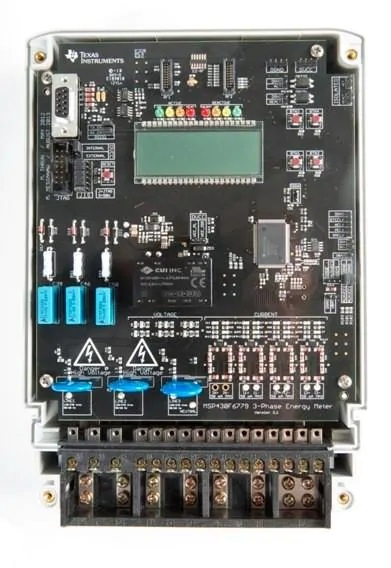
\includegraphics[width = 3cm]{3Proyecto/EVM430-F6779}
            \caption{Tarjeta EVM430-F6779-3} 
            \label{fig:EVM430-F6779-3}
        \end{figure} 
        \begin{itemize}
            \itemsep0em
            \item Es posible ejecutar aplicaciones de medición en tiempo real.
            \item Viene con software de medición.
            \item Se puede conectar a cualquier sistema de prueba o voltaje AC.
            \item Fuentes de alimentación capacitiva y aisladas presentes
            \item Fácil visualización de resultados y calibración a través de RS-232
            \item Pantalla LCD de 160 segmentos
            \item Conectores RF para soporte AMR / AMI
            \item Soporte RTC de 32 kHz (cabecera disponible para calibración RTC)
            \item Encabezados para alimentación MSP430 o solo  RTC a través de fuentes de alimentación auxiliares
        \end{itemize}
    \subsection{EVAL-ADE 7978}
        \begin{figure}[H]
            \centering
            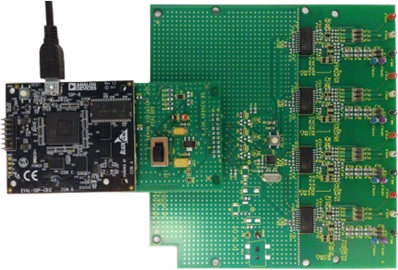
\includegraphics[width = 3cm]{3Proyecto/EVAL-ADE7978}
            \caption{Tarjeta EVAL-ADE7978} 
            \label{fig:EVAL-ADE7978}
        \end{figure}
        \begin{itemize}
            \itemsep0em
            \item Permite sensores Shunt en medidores de energía polifásica. 
            \item Inmune a la manipulación magnética.
            \item Alta precisión; admite EN 50470-1, EN 50470-3, IEC 62053-21, IEC 62053-22, IEC 62053-23, ANSI C12.20, y la estándar IEEE 1459.
            \item Compatible con 3 fases, 3 o 4 lineas (Delta o estrella).
            \item Calcula la energia Activa, Pasiva y Aparente en cada fase y en el sistema general.
            \item Menos del 0.2\% de error en energía activa y reactiva en un rango dinámico de 2000 a 1 a TA = 25$^{\circ}$C
            \item Menos del 0.1\% de error en voltaje rms en un rango dinámico de 500 a 1 a TA = 25$^{\circ}$C.
            \item Menos del 0.25\% de error en corriente rms en un rango dinámico de 500 a 1 a TA = 25$^{\circ}$C.
            \item Mediciones de calidad  de , incluida  la distorsión armónica total (THD).
            \item Suministro de 3.3 V.
            \item Temperatura de funcionamiento: -40$^{\circ}$C a +85$^{\circ}$C. 
            \item Interfaces seriales flexibles I2C, SPI y HSDC.
        \end{itemize}
    \subsection{78M6631 3-Phase PowerMeasurement IC}
        \begin{figure}[H]
            \centering
            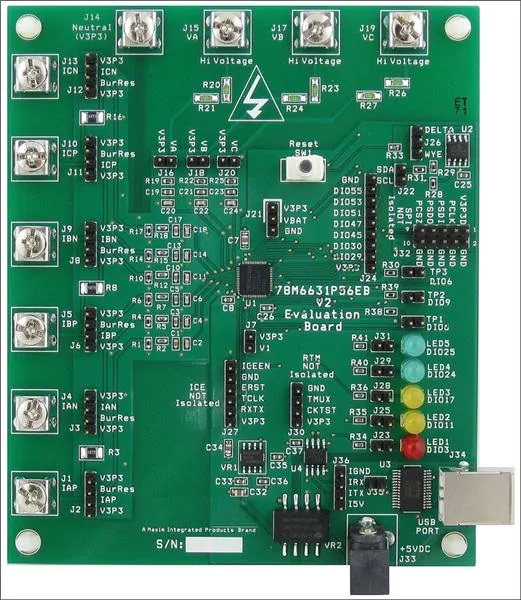
\includegraphics[width = 3cm]{3Proyecto/78M6631-EVM-DSL}
            \caption{Tarjeta 78M6631-EVM-DSL}
            \label{fig:78M6631-EVM-DSL}
        \end{figure}
        \begin{itemize}
            \itemsep0em
            \item 0.5 \% de precisión de vatios sobre 2000 : 1 corriente Rango y temperatura exclusiva
            \item Excede los estándares IEC 62053 / ANSI C12.20.
            \item Referencia de voltaje <40 ppm/ $^{\circ}$C.
            \item Seis entradas analógicas que admiten entradas de medición de corriente y voltaje trifásico.
            \item Configuración delta o estrella.
            \item ADC Delta-Sigma de 22 bits con motor de cómputo (CE) independiente de 32 bits.
            \item MPU de 8 bits (80515), un ciclo de reloj por instrucción con 4 KB MPU XRAM.
            \item 128 KB Flash con seguridad.
            \item Base de tiempo de 32 kHz con temporizador de vigilancia de hardware
            \item Opciones de interfaz de host UART, I2C y High-Speed Slave SPI.
            \item 17 pines I/O tolerante a 5V de uso general.
        \end{itemize}

    Teniendo encenta las características encontradas en las tres tarjetas, se decidió escoger el dispositivo ADE 7978 ya que cumple con la norma IEEE 1459 y tiene una medición precisa, ademas de esto la resolución del dispositivo es mucho mejor que el de los otros ( 24 bits ).

\section{Desarrollo del Hardware}
    \subsection{Configuración inicial}

        La conexión que se realizó, fue una configuración de 3 fases, 4 hilos, distribución estrella. El diagrama de conexión se ve en la figura \ref{fig:configuracion}

        \begin{figure}[H]
            \begin{center}
                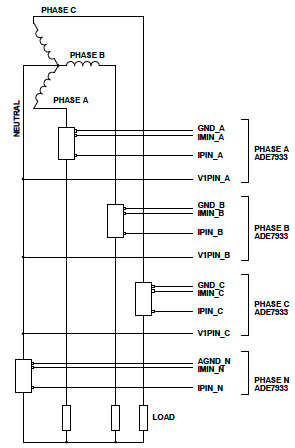
\includegraphics[width = 9cm]{3Proyecto/configuration}
                \caption{ Esquema de conexión para una distribución en Y, 3 fases, 4 hilos.} 
                \label{fig:configuracion}
            \end{center}
        \end{figure}

        \subsubsection{Materiales}
            \begin{itemize}
                \itemsep0em
                \item 4 resistencias Shunt.
                \item 1m de cable 7 hilos 22 AWG azul - V1PIN.
                \item 1m de cable 7 hilos 22 AWG cafe - GND.
                \item 1m de cable 7 hilos 22 AWG amarillo - IMIN.
                \item 1m de cable 7 hilos 22 AWG rojo - IPIN.
                \item 2m de cable duplex 2x10 AWG blanco
                \item 10 TYP UK2.50.
                \item Carril de aluminio.
                \item lamina de acetato.
                \item 20 terminales.
                \item 4 postes Met 10mm.
            
            \end{itemize}

            \begin{figure}[H]
                \begin{center}
                    \includegraphics[width = 3cm]{3Proyecto/Cableado}
                    \caption{ ADE 7978 configurado con las resistencias Shunt} 
                    \label{fig:Cableado}
                \end{center}
            \end{figure}
        Para configurar la tarjeta fue necesario encontrar una resistencia Shunt que se ajustará a las especificaciones del circuito a implementar, sin embargo este trabajo fue mas complicado, ya que las resistencias Shunt disponibles en el mercado son costosas y la mayoría de ellas vienen con resistencias bajas, elevando el voltaje de salida y ampliando el rango de medición del medidor ($\dfrac{I}{R}=V$), se decidió comprar 4 resistencias Shunt caseras las cuales tenían un costo de tan solo \$4.000 COP muy bajo comparado con las importadas o fabricadas industrialmente, en las que su valor esta entre \$50.000 COP - \$ 200.000 COP.\\
        Teniendo todos los materiales, se realiza la conexión de la figura \ref{fig:configuracion}, utilizando el cable azul para el pin V1PIN, el cable café para el pin GND, el cable amarillo para el pin IMIN, el cable rojo para el pin IPIN y el cable blanco para conectar las shunt con el bloque de terminales, todo el montaje puesto sobre una lamina de acetato elevando la tarjeta con los 4 postes Met como se muestra en la figura \ref{fig:Cableado}\\

    \subsection{Caracterizaci\'on de la resistencia Shunt}
        Ya que las resistencias que se compraron son caseras o no tienen una procedencia muy confiable, se realizó la caracterización con los siguientes materiales 
        \subsubsection{Materiales}
            \begin{itemize}
                \itemsep0em
                \item Funente AC fija.
                \item Resistencia lineal variable.
                \item Shunt.
                \item Osciloscopio.
                \item Sonda atenuada de tension.
                \item Sonda de corriente.
            \end{itemize}
        Con estos materiales se crea un circuito para variar la corriente que pasa por la resistencia Shunt, cambiando la resistencia lineal variable, de esta manera se mide la corriente y el voltaje que cae sobre la resistencia figura: \ref{fig:EsquemaCtrShunt}.
        
        \begin{figure}[H]
            \begin{center}
                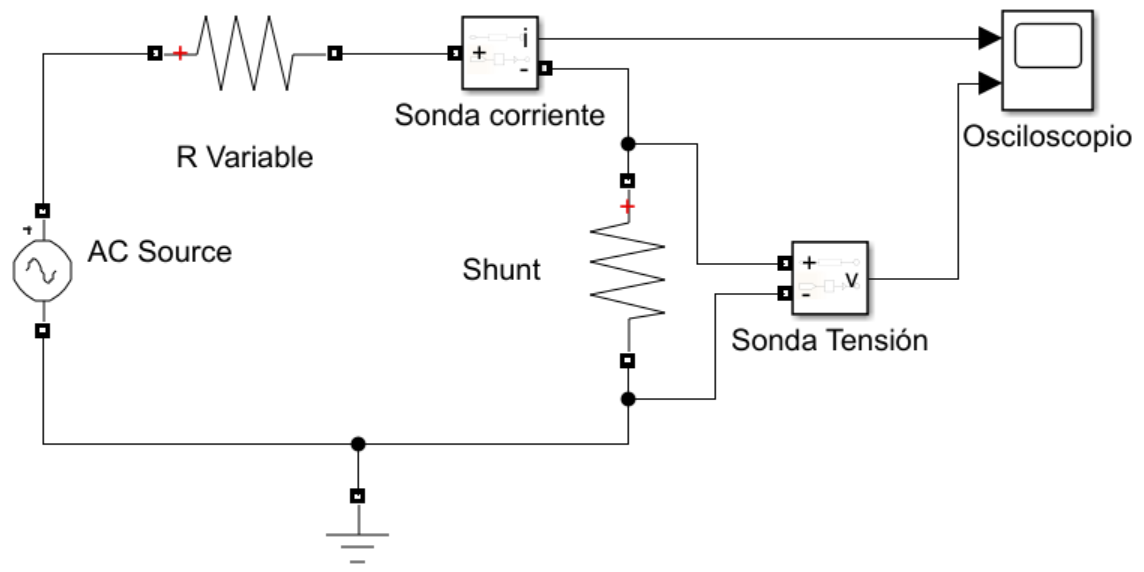
\includegraphics[width = 10cm]{3Proyecto/EsquemaCtrShunt.PNG}
                \caption{ Esquema caracterización de las resistencias Shunt } 
                \label{fig:EsquemaCtrShunt}
            \end{center}
        \end{figure}

        \subsubsection{Shunt A}
            \begin{table} [H]
                \begin{center}
                    \begin{tabular}{ |c|c|c|c|c|c|c|c|c| }
                        \hline 
                        Corriente (A) & 0.552 & 0.558 & 0.565 & 0.566 & 0.575 & 0.583 & 0.586 & 0.597\\
                        \hline
                        Voltaje (V) & 0.00105 & 0.00105 & 0.00107 & 0.00107 & 0.00107 & 0.00108 & 0.00109 & 0.00109\\
                        \hline
                        \hline 
                        Corriente (A) & 0.609 & 0.621 & 0.639 & 0.651 & 0.68 & 0.7 & 0.73 & 0.757\\
                        \hline
                        Voltaje (V) & 0.00111 & 0.00113 & 0.00115 & 0.00117 & 0.0012 & 0.00122 & 0.00125 & 0.0013\\
                        \hline
                        \hline 
                        Corriente (A) & 0.784 & 0.813 & 0.85 & 0.888 & 0.935 & 1.02 & 1.06 & 1.12\\
                        \hline
                        Voltaje (V) & 0.00134 & 0.00136 & 0.00143 & 0.00148 & 0.00153 & 0.00162 & 0.0017 & 0.00179\\
                        \hline
                        \hline 
                        Corriente (A) & 1.21 & 1.28 & 1.38 & 1.45 & 1.59 & 1.63 & 1.75 & 1.8\\
                        \hline
                        Voltaje (V) & 0.0019 & 0.002 & 0.0022 & 0.00226 & 0.00246 & 0.00254 & 0.0027 & 0.00277\\
                        \hline
                        \hline 
                        Corriente (A) & 1.75 & 1.67 & 1.5 & 1.42 & 1.35 & 1.24 & 1.18 & 1.1\\
                        \hline
                        Voltaje (V) & 0.00269 & 0.00257 & 0.00233 & 0.00222 & 0.00211 & 0.00196 & 0.00187 & 0.00176\\
                        \hline
                        \hline 
                        Corriente (A) & 1.06 & 1.01 & 0.97 & 0.92 & 0.879 & 0.84 & 0.816 & 0.777\\
                        \hline
                        Voltaje (V) & 0.00169 & 0.00163 & 0.00158 & 0.00151 & 0.00145 & 0.0014 & 0.00137 & 0.00131\\
                        \hline
                        \hline 
                        Corriente (A) & 0.753 & 0.734 & 0.71 & 0.693 & 0.67 & 0.652 & 0.629 & 0.616\\
                        \hline
                        Voltaje (V) & 0.00127 & 0.00125 & 0.00122 & 0.00119 & 0.00116 & 0.00115 & 0.00112 & 0.00111\\
                        \hline
                        \hline
                        Corriente (A) & 0.605 & 0.591 & 0.575 & 0.562 & 0.555 \\
                        \hline
                        Voltaje (V) & 0.0011 & 0.00108 & 0.00107 & 0.00105 & 0.00104 \\ 
                        \hline
                    \end{tabular}
                \end{center}
                \caption{Corriente vs Voltaje en la resistencia shunt A}
                \label{tab:shuntA}
            \end{table}

            \begin{lstlisting}
                x = [0.552 0.558 0.565 0.566 0.575 0.583 0.586 0.597 0.609 0.621 0.639 0.651 0.68 0.7 0.73 0.757 0.784 0.813 0.85 0.888 0.935 1.02 1.06 1.12 1.21 1.28 1.38 1.45 1.59 1.63 1.75 1.8 1.75 1.67 1.5 1.42 1.35 1.24 1.18 1.1 1.06 1.01 0.97 0.92 0.879 0.84 0.816 0.777 0.753 0.734 0.71 0.693 0.67 0.652 0.629 0.616 0.605 0.591 0.575 0.555 0.562]
                y = [0.00105 0.00105 0.00107 0.00107 0.00107 0.00108 0.00109 0.00109 0.00111 0.00113 0.00115 0.00117 0.0012 0.00122 0.00125 0.0013 0.00134 0.00136 0.00143 0.00148 0.00153 0.00162 0.0017 0.00179 0.0019 0.002 0.0022 0.00226 0.00246 0.00254 0.0027 0.00277 0.00269 0.00257 0.00233 0.00222 0.00211 0.00196 0.00187 0.00176 0.00169 0.00163 0.00158 0.00151 0.00145 0.0014 0.00137 0.00131 0.00127 0.00125 0.00122 0.00119 0.00116 0.00115 0.00112 0.00111 0.0011 0.00108 0.00107 0.00105 0.00104]
                plot( x, y, 'ob', 'markersize', 4, 'markerfacecolor', 'b' ),
                grid,xlabel( 'Corriente ( A )' ), ylabel( 'Voltaje (V)' ),
                title( 'Caracterización de la resistencia Shunt A' )
            \end{lstlisting}

            \begin{figure}[H]
                \begin{center}
                    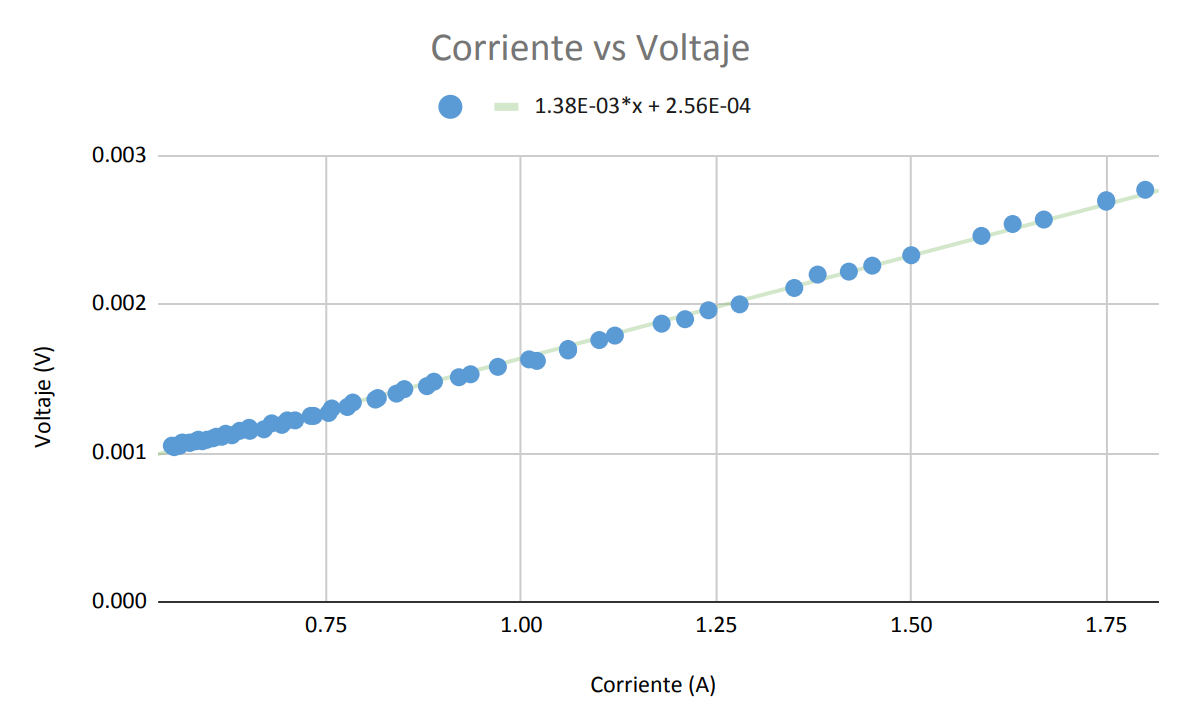
\includegraphics[width = 15cm]{3Proyecto/CorrienteVoltaje1.png}
                    \caption{ Caracterización ShuntA} 
                    \label{fig:Muestras ShuntA}
                \end{center}
            \end{figure}

            Con ayuda de matlab se optine la ecuacion de la recta que mas se ajusta a los datos\\
            donde $V_{out}=$ Voltaje de salida de la Shunt, $I=$ Corriente de entrada a la Shunt 

            \begin{equation}\label{crt ShuntA}
                V_{out} = 0.0013805*I + 0.00025643 
            \end{equation}

        \subsubsection{Shunt B}    
            \begin{table} [H]
                \begin{center}
                    \begin{tabular}{ |c|c|c|c|c|c|c|c|c| }
                        \hline
                        Corriente (A) & 0.549 & 0.574 & 0.606 & 0.633 & 0.67 & 0.698 & 0.744 & 0.77\\
                        \hline
                        Voltaje (V) & 0.00107 & 0.00111 & 0.00112 & 0.00115 & 0.00119 & 0.00125 & 0.0013 & 0.00133\\
                        \hline
                        \hline
                        Corriente (A) & 0.823 & 0.867 & 0.922 & 0.99 & 1.05 & 1.15 & 1.23 & 1.36\\
                        \hline
                        Voltaje (V) & 0.0014 & 0.00145 & 0.00152 & 0.0016 & 0.0017 & 0.00186 & 0.00196 & 0.00213\\
                        \hline
                        \hline
                        Corriente (A) & 1.48 & 1.69 & 1.8 & 1.7 & 1.48 & 1.35 & 1.22 & 1.15\\
                        \hline
                        Voltaje (V) & 0.0023 & 0.0026 & 0.00278 & 0.00262 & 0.0023 & 0.00214 & 0.00194 & 0.00182\\
                        \hline
                        \hline
                        Corriente (A) & 1.05 & 0.977 & 0.913 & 0.85 & 0.811 & 0.76 & 0.728 & 0.685\\
                        \hline
                        Voltaje (V) & 0.0017 & 0.00162 & 0.00151 & 0.00143 & 0.00139 & 0.00132 & 0.00127 & 0.0012\\
                        \hline
                        \hline
                        Corriente (A) & 0.662 & 0.635 & 0.611 & 0.599 & 0.58 & 0.557\\
                        \hline
                        Voltaje (V) & 0.00119 & 0.00116 & 0.00113 & 0.0011 & 0.00109 & 0.00108\\
                        \hline
                    \end{tabular}
                \end{center}
                \caption{Corriente vs Voltaje en la resistencia shunt B}
                \label{tab:shuntB}
            \end{table}

            \begin{lstlisting}
                x = [ 0.549 0.574 0.606 0.633 0.67 0.698 0.744 0.77 0.823 0.867 0.922 0.99 1.05 1.15 1.23 1.36 1.48 1.69 1.8 1.7 1.48 1.35 1.22 1.15 1.05 0.977 0.913 0.85 0.811 0.76 0.728 0.685 0.662 0.635 0.611 0.599 0.58 0.557 ]
                y = [ 0.00107 0.00111 0.00112 0.00115 0.00119 0.00125 0.0013 0.00133 0.0014 0.00145 0.00152 0.0016 0.0017 0.00186 0.00196 0.00213 0.0023 0.0026 0.00278 0.00262 0.0023 0.00214 0.00194 0.00182 0.0017 0.00162 0.00151 0.00143 0.00139 0.00132 0.00127 0.0012 0.00119 0.00116 0.00113 0.0011 0.00109 0.00108 ]
                plot(x,y,'ob','markersize',4,'markerfacecolor','b'),
                grid,xlabel('Corriente (A)'),ylabel('Voltaje (V)'),
                title('Caracterización de la resistencia Shunt B')
            \end{lstlisting}

            \begin{figure}[H]
                \begin{center}
                    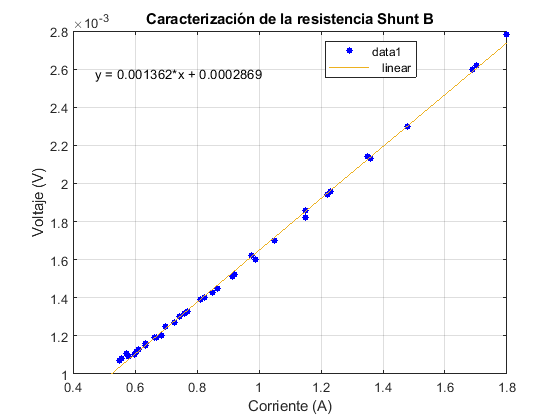
\includegraphics[width = 15cm]{3Proyecto/CorrienteVoltaje2.png}
                    \caption{ Caracterización ShuntB} 
                    \label{fig:Muestras shuntB}
                \end{center}
            \end{figure}

            Con ayuda de matlab se optine la ecuacion de la recta que mas se ajusta a los datos\\
            donde $V_{out}=$ Voltaje de salida de la Shunt, $I=$ Corriente de entrada a la Shunt 

            \begin{equation}\label{crt ShuntB}
                V_{out} = 0.001362*I + 0.0002869 
            \end{equation}

        \subsubsection{Shunt C}

            \begin{table} [H]
                \begin{center}
                    \begin{tabular}{ |c|c|c|c|c|c|c|c|c| }
                        \hline
                        Corriente (A) & 0.557 & 0.573 & 0.593 & 0.631 & 0.654 & 0.69 & 0.717 & 0.752\\
                        \hline
                        Voltaje (V) & 0.00106 & 0.00108 & 0.0011 & 0.00115 & 0.00117 & 0.00122 & 0.00126 & 0.00131\\
                        \hline
                        \hline
                        Corriente (A) & 0.8 & 0.838 & 0.896 & 0.95 & 1.03 & 1.09 & 1.19 & 1.29\\
                        \hline
                        Voltaje (V) & 0.00137 & 0.00141 & 0.00149 & 0.00155 & 0.00166 & 0.00175 & 0.00189 & 0.00205\\
                        \hline
                        \hline
                        Corriente (A) & 1.47 & 1.59 & 1.8 & 1.63 & 1.52 & 1.37 & 1.27 & 1.15\\
                        \hline
                        Voltaje (V) & 0.0023 & 0.00246 & 0.00276 & 0.00251 & 0.00237 & 0.00215 & 0.00199 & 0.00183\\
                        \hline
                        \hline
                        Corriente (A) & 1.07 & 0.98 & 0.925 & 0.86 & 0.816 & 0.766 & 0.737 & 0.697\\
                        \hline
                        Voltaje (V) & 0.00172 & 0.0016 & 0.00153 & 0.00144 & 0.00138 & 0.00131 & 0.0013 & 0.00121\\
                        \hline
                        \hline
                        Corriente (A) & 0.661 & 0.633 & 0.616 & 0.599 & 0.558\\
                        \hline
                        Voltaje (V) & 0.00119 & 0.00115 & 0.00113 & 0.00111 & 0.00107\\
                        \hline
                    \end{tabular}
                \end{center}
                \caption{Corriente vs Voltaje en la resistencia shunt C}
                \label{tab:shuntC}
            \end{table}

            \begin{lstlisting}
                x = [ 0.557 0.573 0.593 0.631 0.654 0.69 0.717 0.752 0.8 0.838 0.896 0.95 1.03 1.09 1.19 1.29 1.47 1.59 1.8 1.63 1.52 1.37 1.27 1.15 1.07 0.98 0.925 0.86 0.816 0.766 0.737 0.697 0.661 0.633 0.616 0.599 0.558 ]
                y = [ 0.00106 0.00108 0.0011 0.00115 0.00117 0.00122 0.00126 0.00131 0.00137 0.00141 0.00149 0.00155 0.00166 0.00175 0.00189 0.00205 0.0023 0.00246 0.00276 0.00251 0.00237 0.00215 0.00199 0.00183 0.00172 0.0016 0.00153 0.00144 0.00138 0.00131 0.0013 0.00121 0.00119 0.00115 0.00113 0.00111 0.00107 ]
                plot(x,y,'ob','markersize',4,'markerfacecolor','b'),
                grid,xlabel('Corriente (A)'),ylabel('Voltaje (V)'),
                title('Caracterización de la resistencia Shunt C')
            \end{lstlisting}


            \begin{figure}[H]
                \begin{center}
                    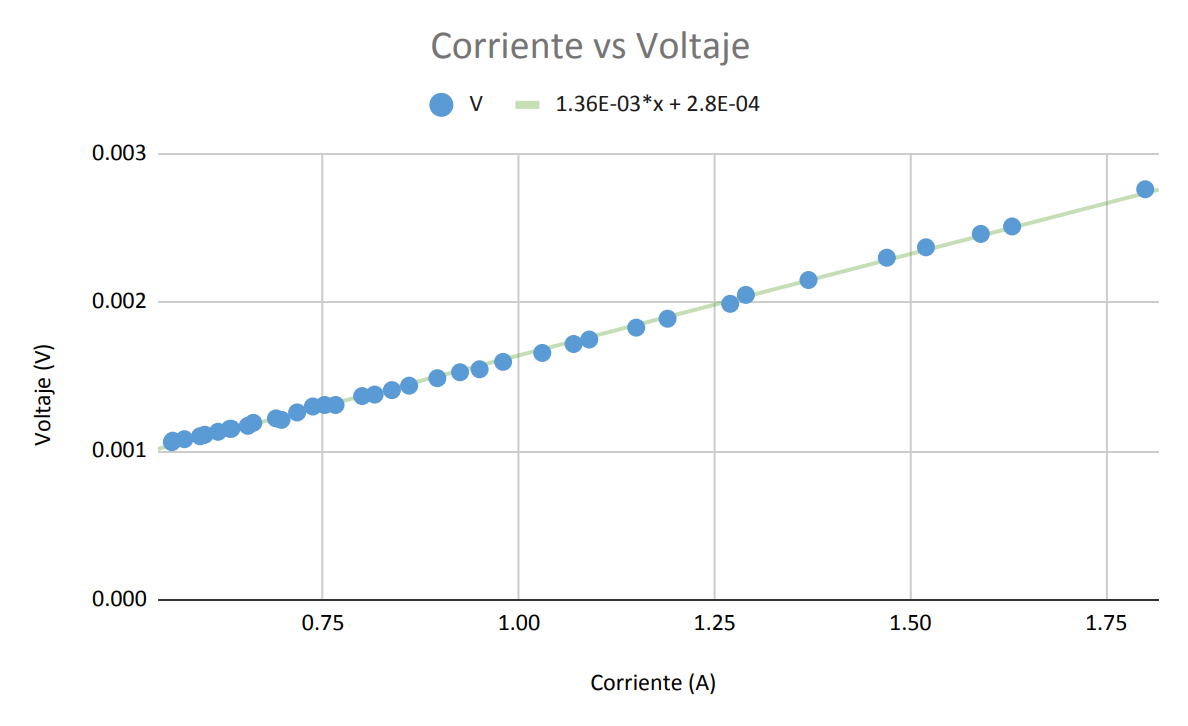
\includegraphics[width = 15cm]{3Proyecto/CorrienteVoltaje3.png}
                    \caption{ Caracterización ShuntC} 
                    \label{fig:Muestras shuntC}
                \end{center}
            \end{figure}
            
            Con ayuda de matlab se optine la ecuacion de la recta que mas se ajusta a los datos\\
            donde $V_{out}=$ Voltaje de salida de la Shunt, $I=$ Corriente de entrada a la Shunt 

            \begin{equation}\label{crt ShuntC}
                V_{out} = 0.0013634*I + 0.00027985 
            \end{equation}

    \subsection{Conversión de voltaje}
        Para obtener el voltaje de entrada del ADE7978, se realizaron los siguientes pasos:\\

        La carga se conecta a la fase siguiendo el diagrama de conexión \ref{fig:configuracion}. Los pines V1PIN y GND\_A, pasan por un divisor de voltaje donde su salida es el pin V1P y VM como se ve en la figura \ref{fig:divisorVolate}. El divisor se modela bajo la siguiente ecuación:\\

        \begin{equation}
            V1P = \frac{R_{2}}{R_{1} + R_{2}} * V_{in}
        \end{equation}

        Donde $\; R1 = 990150 \ohm$, \;$R2 = 1 K\ohm$.\\

        \begin{equation}\label{divisorVoltaje}
            V1P = 0.00100893 * V_{in}
        \end{equation}

        El divisor de voltaje es necesario ya que el conversor ADE7933 solo debe recibir valores en un rango de $\pm 0.5V$. 

        El voltaje VA es la diferencia de voltaje que hay entre V1P y VM, esta es la señal que el conversor transforma a digital. La salida digital que entrega el conversor tiene un rango de $\pm 5.320.000$ como se ve en la figura \ref{fig:voltageOutput}. Esta señal entra al ADE7978 y de ahí en adelante, todos los procesos que se ejecutan, son basados en la conversión anteriormente descrita.\\

        La relación de entrada y salida del conversor ADE7933, consiste en un voltaje pico de entrada de $0.5 V$, genera una señal de salida de $5.320.000$.\\

        La siguiente ecuación relaciona la señal de salida del conversor con la señal de entrada al medidor:\\

        \begin{align*}
            &0,5V \rightarrow 5,320,000.\\
            &V1P \rightarrow DRV
        \end{align*}

        Donde $DRV = Dato\;del\;rango\;de\;voltaje\;del\;conversor$\\

        \begin{equation}
            V1P = \frac{DRV * 0.5}{5.320.000}
        \end{equation}

        \begin{equation}\label{relacionConversor}
            V1P = DRV * 9,39845 * 10^{-8} 
        \end{equation}

        Reemplazando la ecuación del divisor de voltaje \ref{divisorVoltaje} en \ref{relacionConversor}

        \begin{align*}
            0.00100893 * V_{in} = DRV * 9,39845 * 10^{-8} 
        \end{align*}

        \begin{equation}\label{conversorEntradaSalida}
            V_{in} = DRV * 0,00009315311
        \end{equation}
        La ecuación \ref{conversorEntradaSalida} modela la relación del voltaje de entrada al circuito al rango de voltaje del conversor.

        \begin{figure}[H]
            \centering
            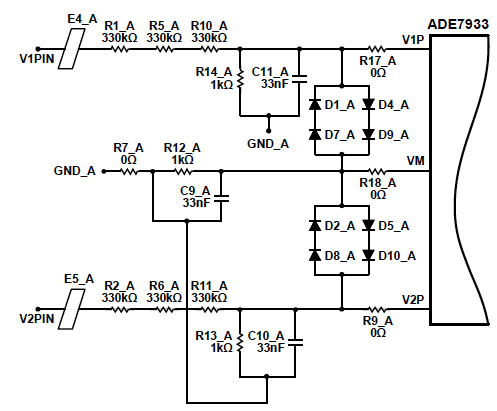
\includegraphics[width = 10cm]{3Proyecto/divisorVoltaje}
            \caption{Divisor de voltaje ADC} 
            \label{fig:divisorVolate}
        \end{figure} 

        \begin{figure}[H]
            \centering
            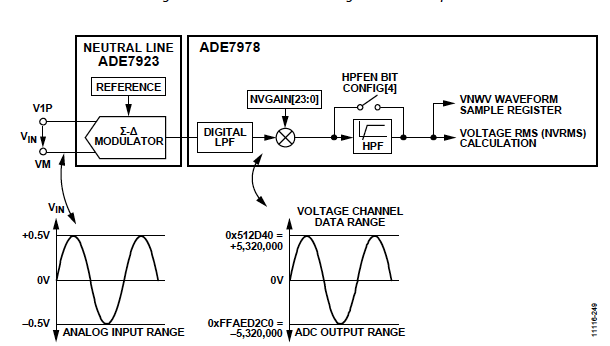
\includegraphics[width = 10cm]{3Proyecto/voltageOutput}
            \caption{Salida de voltaje del ADE 7978} 
            \label{fig:voltageOutput}
        \end{figure} 


    \subsection{Conversión de corriente}
        Para encontrar la relación que hay entre la entrada de corriente y el convertidor ADC fue necesario utilizar la ecuación de la recta arrojada por las muestras de la caracterización de las shunt y también fue necesario hallar la relación de voltaje entre el pin IP e IM que son los usados por el ADC para convertir la señal figura \ref{fig:CircuitoCorriente}


        \begin{figure}[H]
            \begin{center}
                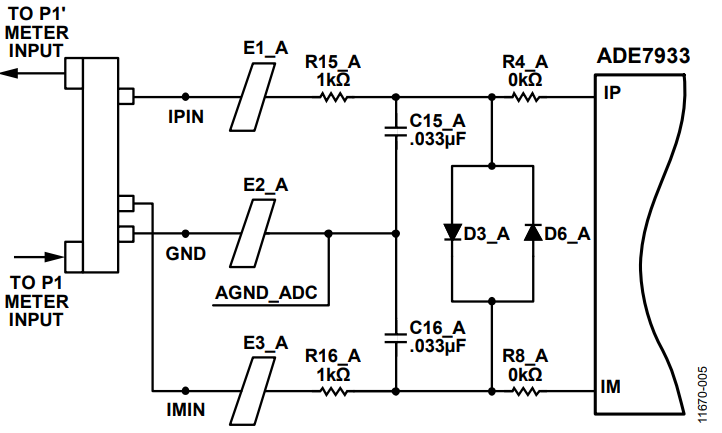
\includegraphics[width = 10cm]{3Proyecto/CircuitoCorriente.PNG}
                \caption{ Circuito de protección para los pines IP e IM } 
                \label{fig:CircuitoCorriente}
            \end{center}
        \end{figure}

        Como ya se tiene la relación entre la corriente de entrada y el voltaje de salida en la Shunt se procede hallar el voltaje entre el pin IP e IM resolviendo el circuito por medio del teorema de nodos como se muestra en la figura \ref{fig:Nodos}, los diodos de protección se eliminan ya que la tarjeta viene sin ellos de fabrica. \\

        Para simplificar el circuito electrónico se remplaza el filtro de ferrita con la resistencia de 1k por R1, como el valor de los condensadores es el mismo, ambos condensadores se simbolizan con la letra C \ref{fig:Nodos}.

        \begin{figure}[H]
            \begin{center}
                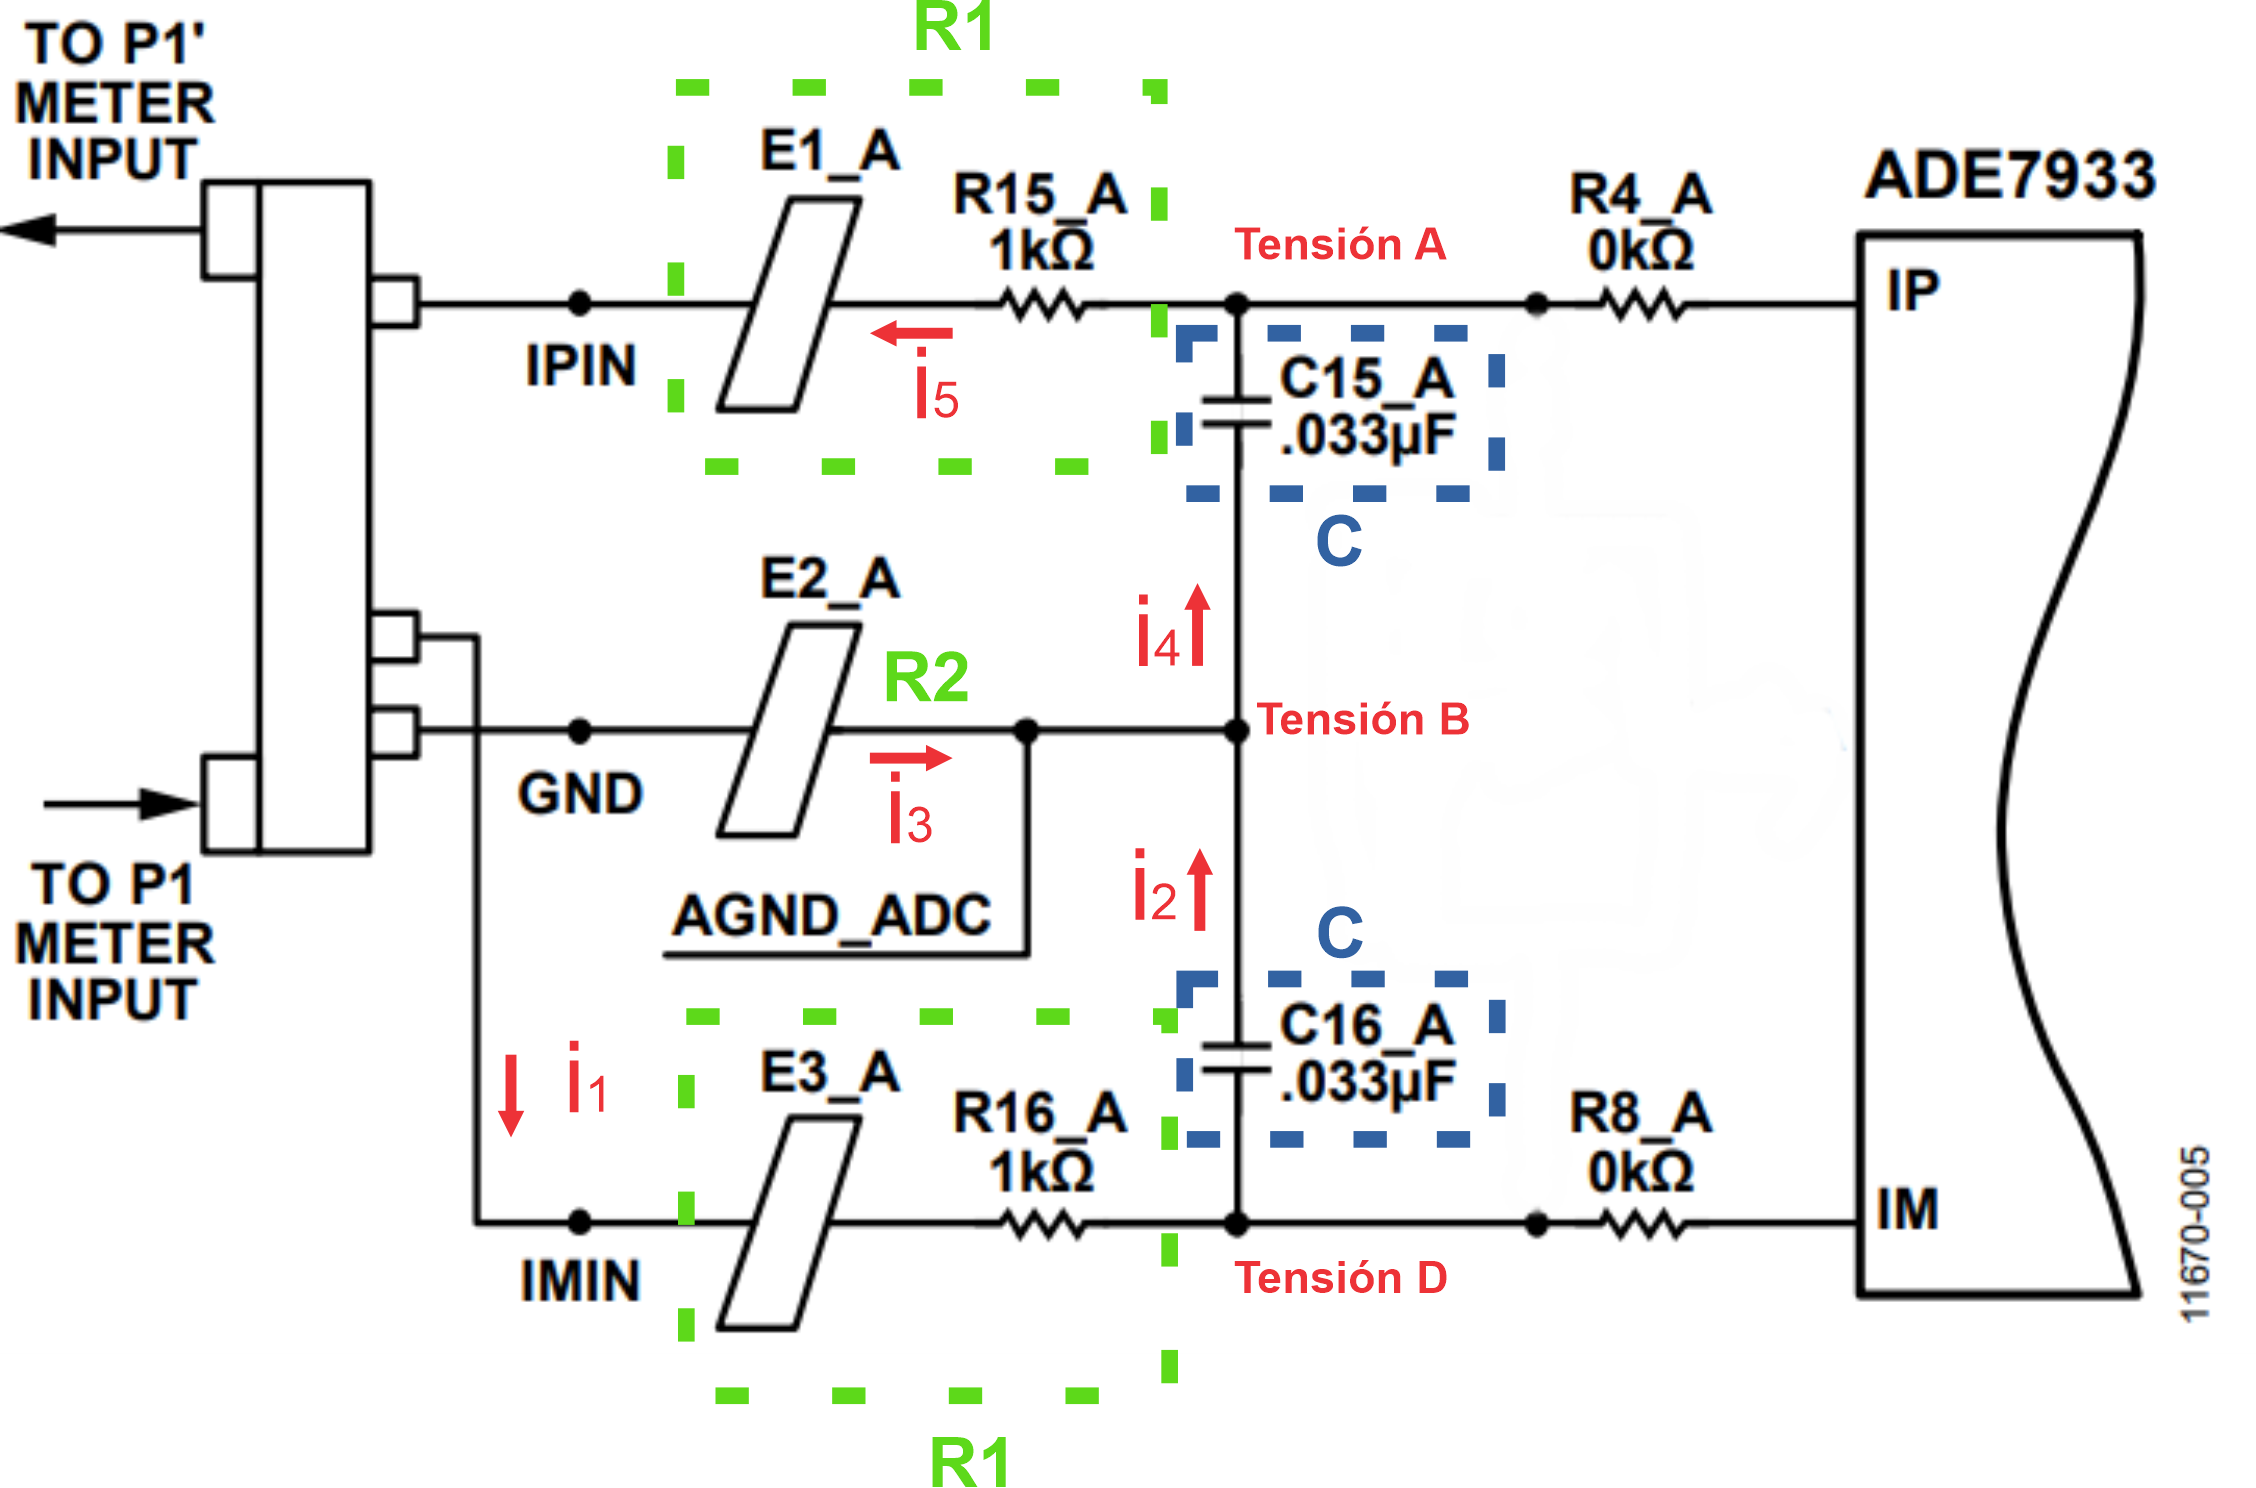
\includegraphics[width = 10cm]{3Proyecto/Nodos.PNG}
                \caption{ Nodos aplicados al circuito} 
                \label{fig:Nodos}
            \end{center}
        \end{figure}

        Se asume que el circuito se alimenta con una fuente de voltaje AC con terminal $+$ en GND e IMIN y terminal $-$ en IPIN resolviendolo de la siguiente manera :
        \\  

        \begin{itemize}
            \item \textbf{Tensión D} \\
            $\mathbf{i_{1}=i_{2}}$
            \begin{align*}
                &\frac{V_{i}}{R_{1}}-\frac{D}{R_{1}} = \frac{D}{ZC}-\frac{B}{ZC} \\\\
                &\frac{B}{ZC} = \frac{D}{ZC}- \frac{V_{i}}{R_{1}} + \frac{D}{R_{1}} \\\\
                &\frac{B}{ZC} = D(\frac{1}{ZC} +\frac{1}{R_{1}}) - \frac{V_{i}}{R_{1}} \\\\
                &\frac{B}{ZC} = D\frac{R_{1}+ZC}{R_{1}ZC} - \frac{V_{i}}{R_{1}} \\\\
            \end{align*}
            \begin{equation}\label{Nodo D}
                B = D\frac{R_{1}+ZC}{R_{1}} - V_{i}\frac{ZC}{R_{1}}
            \end{equation}
                \item \textbf{Tensión B} \\
                $ \mathbf{i_{2} + i_{3} = i_{4}}$
                \begin{align*}
                    &\frac{D}{ZC} - \frac{B}{ZC} + \frac{V_{i}}{R_{2}}-\frac{B}{R_{2}} = \frac{B}{ZC} - \frac{A}{ZC}\\\\
                    &\frac{D}{ZC}  + \frac{V_{i}}{R_{2}} + \frac{A}{ZC} = B\frac{2}{ZC}  + \frac{B}{R_{2}} \\\\
                    &\frac{D}{ZC}  + \frac{V_{i}}{R_{2}} + \frac{A}{ZC} = B(\frac{2}{ZC}  + \frac{1}{R_{2}}) \\\\
                    &\frac{D}{ZC}  + \frac{V_{i}}{R_{2}} + \frac{A}{ZC} = B\frac{2R_{2}+ZC}{R_{2}ZC}
                \end{align*}
                \begin{equation}\label{Nodo B}
                    D\frac{R_{2}}{2R_{2}+ZC}  + V_{i}\frac{ZC}{2R_{2}+ZC} + A\frac{R_{2}}{2R_{2}+ZC} = B
                \end{equation}
                \item \textbf{Tensión A} \\
                $ \mathbf{i_{4}=i_{5}}$
                \begin{align*}
                    &\frac{B}{ZC} - \frac{A}{ZC} = \frac{A}{R_{1}}\\\\
                    &\frac{B}{ZC} = \frac{A}{R_{1}} + \frac{A}{ZC}\\\\
                    &\frac{B}{ZC} = A(\frac{1}{R_{1}} + \frac{1}{ZC})\\\\
                    &\frac{B}{ZC} = A\frac{R_{1}+ZC}{R_{1}ZC}
                \end{align*}
                \begin{equation}\label{Nodo A}
                    B= A\frac{R_{1}+ZC}{R_{1}} \\\\
                \end{equation}
        \end{itemize}
    
        Remplazando la ecuación de Tensión D \ref{Nodo D} en la ecuación de tensión B \ref{Nodo B}
        \begin{align*}
            &D\frac{R_{1}+ZC}{R_{1}} - V_{i}\frac{ZC}{R_{1}} = D\frac{R_{2}}{2R_{2}+ZC}  + V_{i}\frac{ZC}{2R_{2}+ZC} + A\frac{R_{2}}{2R_{2}+ZC} \\\\
            &A\frac{R_{2}}{2R_{2}+ZC} = D\frac{R_{1}+ZC}{R_{1}} - V_{i}\frac{ZC}{R_{1}} - D\frac{R_{2}}{2R_{2}+ZC} - V_{i}\frac{ZC}{2R_{2}+ZC}  \\\\
            &A\frac{R_{2}}{2R_{2}+ZC} = D(\frac{R_{1}+ZC}{R_{1}} - \frac{R_{2}}{2R_{2}+ZC}) - V_{i}(\frac{ZC}{R_{1}}  + \frac{ZC}{2R_{2}+ZC}) \\\\
            &A\frac{R_{2}}{2R_{2}+ZC} = D\frac{(R_{1}+ZC)(2R_{2}+ZC)-R_{1}R_{2}}{R_{1}(2R_{2}+ZC)} - V_{i}\frac{ZC(2R_{2}+ZC)+ R_{1}ZC}{R_{1}(2R_{2}+ZC)} \\\\
        \end{align*}
        \begin{equation}\label{Nodo D en B}
            A = D\frac{ (R_{1}+ZC)(2R_{2}+ZC)-R_{1}R_{2} }{ R_{1}R_{2}} - V_{i}\frac{ ZC(2R_{2}+ZC)+ R_{1}ZC }{ R_{1}R_{2}}
        \end{equation}
    
        Remplazando la ecuación de tensión D \ref{Nodo D} en la ecuación de tensión A \ref{Nodo A}
        \begin{align*}
            &D\frac{R_{1}+ZC}{R_{1}} - V_{i}\frac{ZC}{R_{1}} = A\frac{R_{1}+ZC}{R_{1}} \\\\
        \end{align*}
        \begin{equation}\label{Nodo D en A}
            A = D - V_{i}\frac{ZC}{R_{1}+ZC}
        \end{equation}
    
        Remplazando la ecuación \ref{Nodo D en B} en la ecuación \ref{Nodo D en A} para dejar D en términos de $V_{i}$
        \begin{align*}
            &D\frac{ (R_{1}+ZC)(2R_{2}+ZC) - R_{1}R_{2} }{ R_{1}R_{2}} - V_{i}\frac{ ZC(2R_{2}+ZC)+ R_{1}ZC }{ R_{1}R_{2}} = D - V_{i}\frac{ZC}{R_{1}+ZC} \\\\
            &D\frac{ (R_{1}+ZC)(2R_{2}+ZC) -  R_{1}R_{2} }{ R_{1}R_{2}} - D = V_{i}\frac{ ZC(2R_{2}+ZC)+ R_{1}ZC }{ R_{1}R_{2}} - V_{i}\frac{ZC}{R_{1}+ZC} \\\\
            &D(\frac{ (R_{1}+ZC)(2R_{2}+ZC) -  R_{1}R_{2} }{ R_{1}R_{2} } - 1) = V_{i}(\frac{ ZC(2R_{2}+ZC)+ R_{1}ZC }{ R_{1}R_{2}} - \frac{ZC}{R_{1}+ZC}) \\\\
            &D(\frac{ (R_{1}+ZC)(2R_{2}+ZC) -  2R_{1}R_{2} }{ R_{1}R_{2} }) = V_{i}\frac{ [ZC(2R_{2}+ZC)+ R_{1}ZC][R_{1}+ZC] - R_{1}R_{2}ZC }{ R_{1}R_{2}(R_{1}+ZC)} \\\\
        \end{align*}
        \begin{equation}\label{Final D en funcion de Vi}
            D = V_{i}\frac{ [ZC(2R_{2}+ZC)+ R_{1}ZC][R_{1}+ZC] - R_{1}R_{2}ZC }{ [(R_{1}+ZC)(2R_{2}+ZC) -  2R_{1}R_{2}][R_{1}+ZC]} \\\\
        \end{equation}
    
        Remplazando \ref{Final D en funcion de Vi} en la ecuación \ref{Nodo D en A} para obtener A en términos de $V_{i}$
        \begin{align*}
            &A = V_{i}\frac{ [ZC(2R_{2}+ZC)+ R_{1}ZC][R_{1}+ZC] - R_{1}R_{2}ZC }{ [(R_{1}+ZC)(2R_{2}+ZC) -  2R_{1}R_{2}][R_{1}+ZC]} - V_{i}\frac{ZC}{R_{1}+ZC}\\\\
            &A = V_{i}(\frac{ [ZC(2R_{2}+ZC)+ R_{1}ZC][R_{1}+ZC] - R_{1}R_{2}ZC }{ [(R_{1}+ZC)(2R_{2}+ZC) -  2R_{1}R_{2}][R_{1}+ZC]} - \frac{ZC}{R_{1}+ZC})\\\\
        \end{align*}

        \small
        \begin{equation}\label{Final A en funcion de Vi}
            \begin{aligned}
                & A = V_{i} *\\\\
                & \frac{ ([ZC(2R_{2}+ZC)+ R_{1}ZC][R_{1}+ZC] - R_{1}R_{2}ZC)(R_{1}+ZC) - ZC[(R_{1}+ZC)(2R_{2}+ZC) -  2R_{1}R_{2}][R_{1}+ZC] }{ [(R_{1}+ZC)(2R_{2}+ZC) -  2R_{1}R_{2}][R_{1}+ZC][R_{1}+ZC] }\\
            \end{aligned}
        \end{equation}
        \normalsize
    
        Con ayuda del software Matlab se remplazan los valores y se resuelve la ecuación D y A

        \begin{lstlisting}
            
            R1 = 1150;
            R2 = 150;
            f = 60;
            W = 2*pi*f;
            C = 33*10^(-9);
            ZC = -j/(W*C);

            NumD = ( ZC*(2*R2+ZC) + R1*ZC )*(R1+ZC)-R1*R2*ZC
            DenD = ((R1+ZC)*(2*R2+ZC)-2*R1*R2)*(R1+ZC)
            D= NumD/DenD

            NumA = ((ZC*(2*R2+ZC)+R1*ZC)*(R1+ZC)-R1*R2*ZC)*(R1+ZC)-ZC *
                    ((R1+ZC)*(2*R2+ZC)-2*R1*R2)*(R1+ZC)
            DenA = ((R1+ZC)*(2*R2+ZC)-2*R1*R2)*(R1+ZC)*(R1+ZC)
            A= NumA/DenA
        \end{lstlisting}

        \begin{equation}\label{Tension D}
            D = V_{ i }( 1.0000 - 0.0000j)
        \end{equation}
        \begin{equation}\label{Tension A}
            A = V_{ i }( 0.0002 + 0.0143j)
        \end{equation}
        
        El voltaje que le entra a la tarjeta es la diferencia entre la tensión D y la tensión A

        \begin{lstlisting}
            VIMIP = D-A
        \end{lstlisting}

        \begin{equation}\label{Tension V IM-IP}
            V_{IM-IP} = V_{ i }( 0.9998 - 0.0143j)
        \end{equation}

        
        Usando la relación entre corriente y voltaje de las Shunt ecuaciones ( \ref{crt ShuntA},\ref{crt ShuntB}, \ref{crt ShuntC}) se remplaza para despejar la ecuación en términos de corriente y voltaje entre IM-IP
        \begin{itemize}
            \item \textbf{Shunt A} 
                \begin{equation}\label{Tension V IM-IP}
                    V_{IM-IP} = (0.0013805*I + 0.00025643)( 0.9998 - 0.0143j)
                \end{equation}
            \item \textbf{Shunt B} 
                \begin{equation}\label{Tension V IM-IP}
                    V_{IM-IP} = (0.001362*I + 0.0002869)( 0.9998 - 0.0143j)
                \end{equation}
            \item \textbf{Shunt C} 
                \begin{equation}\label{Tension V IM-IP}
                    V_{IM-IP} = (0.0013634*I + 0.00027985)( 0.9998 - 0.0143j)
                \end{equation}
        \end{itemize}

        \begin{figure}[H]
            \begin{center}
                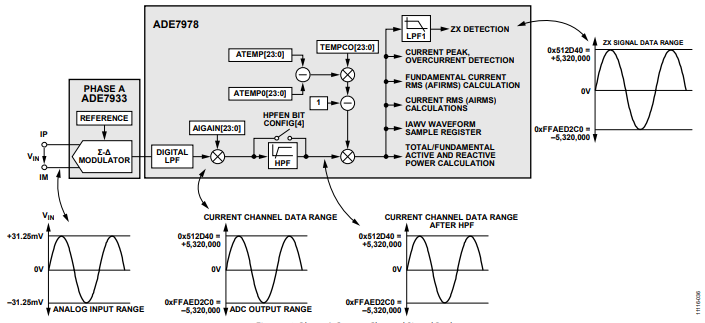
\includegraphics[width = 15cm]{3Proyecto/ConversorCorrienteADE.PNG}
                \caption{ Relacion ADC corriente} 
                \label{fig:Relacion ADC corriente}
            \end{center}
        \end{figure}

        Teneniendo encuenta la conversion de salida del ADC figura \ref{fig:Relacion ADC corriente} se halla la relacion entre corriente y salida del conversor con la ecuacion
        
        \begin{align*}
            &31.25mV \rightarrow 5,320,000.\\
            &V_{IM-IP} \rightarrow DRI
        \end{align*}

        Donde $DRI = Dato\;del\;rango\;de\;corriente\;del\;conversor$\\

        \begin{equation}\label{relacionConversorCorriente}
            V_{IM-IP} = \frac{DRI * 0.03125}{5.320.000}
        \end{equation}

        \begin{itemize}
            \item \textbf{Shunt A} 
                \begin{equation}\label{Tension V IM-IP}
                    \frac{DRI * 0.03125}{5.320.000} = (0.0013805*I + 0.00025643)( 0.9998 - 0.0143j)
                \end{equation}
            \item \textbf{Shunt B} 
                \begin{equation}\label{Tension V IM-IP}
                    \frac{DRI * 0.03125}{5.320.000} = (0.001362*I + 0.0002869)( 0.9998 - 0.0143j)
                \end{equation}
            \item \textbf{Shunt C} 
                \begin{equation}\label{Tension V IM-IP}
                    \frac{DRI * 0.03125}{5.320.000} = (0.0013634*I + 0.00027985)( 0.9998 - 0.0143j)
                \end{equation}
        \end{itemize}
        
        Con ayuda de Matlab se resuelve la ecuacion dejandola en términos de $I = f(ADCI) $.
        \begin{itemize}
            \item \textbf{Shunt A} 
                \begin{lstlisting}
                eqn=(0.0013805*I + 0.00025643 )*VIPIM == ADCI*0.03125/5320000
                solveI=solve(eqn,I)
                \end{lstlisting}
                \begin{align*}
                    &I = ADCI*( 4.2550e^{ -6}  + 6.0876e^{ -8 }j ) - 1.8575e^{ -1 }
                \end{align*}
                Esta expresión es la que se iba a usar para convertir la salida del ADCI en términos de corriente, pero como la Rasberry Pi no acepta números imaginarios, es necesario tener una constate de multiplicación para la conversión.
                \\
                Para resolver esto, se decidió despreciar la parte imaginaria ya que tiene un valor muy pequeño comparado con la parte real
                \begin{equation}\label{Cnt conversion ShuntA}
                    I = 4.2550e^{ -6 }*ADCI - 1.8575e^{ -1 }
                \end{equation}
            \item \textbf{Shunt B} 
                \begin{lstlisting}
                eqn=(0.001362*I+0.0002869 )*VIPIM == ADCI*0.03125/5320000
                solveI=solve(eqn,I)
                \end{lstlisting}
                \begin{align*}
                    &I = ADCI( 4.3128e^{ -6 } + 6.1703e^{ -8 }i ) - 2.1065e^{ -1 }
                \end{align*}
                En la Shunt B tambien se cumple la misma condicion de la Shunt A. 
                \begin{equation}\label{Cnt conversion ShuntB}
                    I = 4.3128e^{ -6 }*ADCI - 2.1065e^{ -1 }
                \end{equation}
            \item \textbf{Shunt C} 
                \begin{lstlisting}
                eqn=(0.0013634*I + 0.00027985 )*VIPIM == ADCI*0.03125/5320000
                solveI=solve(eqn,I)
                \end{lstlisting}
                \begin{align*}
                    &I = ADI*( 4.3084e^{ -6 } + 6.1639e^{ -8} i ) - 2.0526e^{ -1 }
                \end{align*}
                En la Shunt C tambien se cumple la misma condicion de la Shunt A. 
                \begin{equation}\label{Cnt conversion ShuntC}
                    I = 4.3084e^{ -6 }*ADCI - 2.0526e^{ -1 }
                \end{equation}
        \end{itemize}
    
\section{Desarrollo de Software}
    \subsection{Implementación del protocolo I2C entre la rasberry y el ADE7978}

        El protocolo I2C es un estandar internacional para la comunicacion entre dispositivos. Siguiendo la teoria de comunicación I2C se conectó GPIO de la rasberry con el puerto de comunicación del ADE7978 como se muestra en la figura 
        \ref{fig:Coneccion I2C}\\
        \begin{figure}[H]
            \begin{center}
                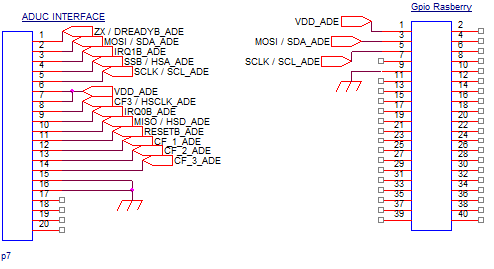
\includegraphics[width = 15cm]{3Proyecto/I2Cconnection.png}
                \caption{ Conexión I2C } 
                \label{fig:Coneccion I2C}
            \end{center}
        \end{figure}

        El puerto de comunicacion del ADE7978 funciona 100\% como un esclavo a un clock maximo de 400kHz; en la operación de escritura se envia un bit en 0  para indicar que la operación va a iniciar, seguido de la dirección del dispositivo que es de 8 bits, seguido de la dirección del registro que se quiere escribir y por ultimo la información que se quiere escribir en el registro fig: \ref{fig:I2C protocol write}; para la operación de lectura se debe envia un 0 para indicar que la operación va a iniciar, seguido de la dirección del dispositivo y la dirección del registro que se quiere leer, seguido de otro bit en 0 y la dirección del dispositivo nuevamente, en ese momento se empieza a recibir la información que esta alojada en ese registro fig: \ref{fig:I2C protocol read}.
        
        \begin{figure}[H]
            \begin{center}
                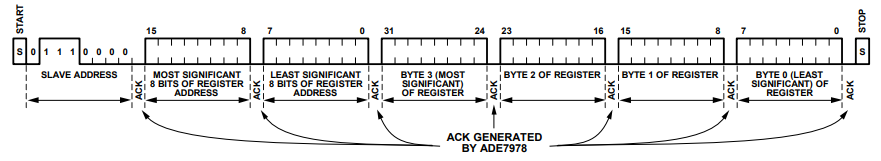
\includegraphics[width = 15cm]{3Proyecto/I2CProtocol.PNG}
                \caption{ Protocolo de escritura I2C} 
                \label{fig:I2C protocol write}
            \end{center}
        \end{figure}
        \begin{figure}[H]
            \begin{center}
                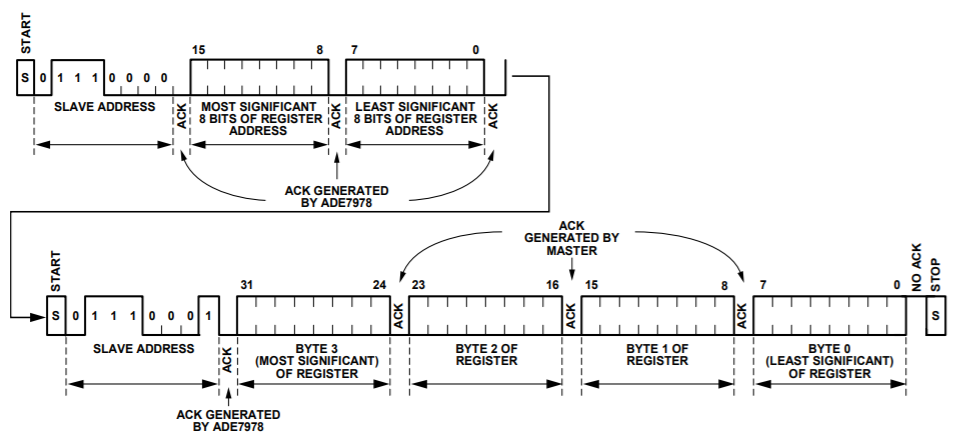
\includegraphics[width = 15cm]{3Proyecto/I2CProtocolRead.PNG}
                \caption{ Protocolo de lectura I2C} 
                \label{fig:I2C protocol read}
            \end{center}
        \end{figure}

        Con la teoria obtenida del datasheet, se realizó la programación de esta comunicación por medio del lenguaje c++, usando la libreria BCM2835 \cite{A40}, a esta libreria fue necesario realizarle un cambio en la función de lectura del puerto I2C, ya que esta libreria está desarrollada para enviar direcciónes de registro de solo 8 bits y en el caso del ADE 7978 cada dirección de registro es de 16 bits, esta modificacion se realizó en el método \textbf{bcm2835 i2c read register rs} agregandole un segundo carácter al la operaciónde envio de la siguiente manera :
        \begin{lstlisting}
        /* Clear FIFO */
        bcm2835_peri_set_bits(control, BCM2835_BSC_C_CLEAR_1 , BCM2835_BSC_C_CLEAR_1 );
        /* Clear Status */
        bcm2835_peri_write(status, BCM2835_BSC_S_CLKT | BCM2835_BSC_S_ERR | BCM2835_BSC_S_DONE);
        /* Set Data Length */
        bcm2835_peri_write(dlen, 1);
        /* Enable device and start transfer */
        bcm2835_peri_write(control, BCM2835_BSC_C_I2CEN);
        bcm2835_peri_write(fifo, regaddr[1]);
        bcm2835_peri_write(fifo, regaddr[0]);
        bcm2835_peri_write(control, BCM2835_BSC_C_I2CEN | BCM2835_BSC_C_ST);
        \end{lstlisting}

        Teniendo el codigo editado, se instaló la libreria como lo recomienda el fabrincante, una vez instalada la libreria se desarrolló la primera parte de la comunicacion en c++ tomando como ejemplo la comunicacion que realiza el mismo fabricante
        \begin{itemize}
            \item Importar la libreria bcm2835.h
            \item Iniciar el puerto puerto de pines de la rasberry
            \item Iniciar el puerto de comunicacion I2C
            \item Cargar la dirección del dispositivo esclavo
            \item Cargar la frecuencia del clock
            \item Llamar el método de lectura pasandole la dirección del regustro, bus de datos y la longitud del mismo
            \item Terminar la comunicacion del puerto I2C y del puerto de la rasberry
        \end{itemize}
        Con estos pasos ya se optiene el dato en el bus, el codigo de los pasos es el siguiente:

        \begin{lstlisting}
            //iniciar puerto raspberry
            //bcm2835_init();
            init = I2C_BEGIN;
            if (!bcm2835_init())
            {
                printf("Falló bcm2835_init, corra el programa con permisos de administrador\n"); //("bcm2835_init failed. Are you running as root??\n");
            }
            // I2C begin if specified
            if (init == I2C_BEGIN)
            {
                if (!bcm2835_i2c_begin())
                {
                    printf("Falló bcm2835_begin, corra el programa con permisos de administrador\n"); //("bcm2835_i2c_begin failed. Are you running as root??\n");
                }
            }
            //Cargar dirección del esclavo
            bcm2835_i2c_setSlaveAddress(slave_address);
            //Cargar la frecuencia del clock
            bcm2835_i2c_setClockDivider(clk_div);

            //Cargar variable buf con el Value
            bcm2835_i2c_read_register_rs(dir, buf, Len_dato);
            //termina la comunicación para no sobresaturar el puerto
            bcm2835_i2c_end();
            bcm2835_close();
        \end{lstlisting}

        
        \subsection{Backend Solución en c++}
            Con la prueba exitosa se comienzó a desarrollar toda la logica del programa para tomar todos los registros de la DSP
            \begin{itemize}
                \item Se creó una clase que contenga todas las propiedades y métodos que describan el funcionamiento de los registros
                \item Crear un objeto de la clase creada por cada registro de la DSP
                \item Crear funciones dentro del programa que permitan la manipulacion y el analisis de dichos registros
                \item Mantener el programa principal en un bucle infinito para que siempre se ejecute.
            \end{itemize}

            Se creó una clase con el nombre Registro conteniendo las siguientes propiedades y métodos
            \subsubsection{Propiedades}
                \begin{itemize}
                    \item Address: dirección en exadecimal del la posición en memoria del registro.
                    \item Len dato: tamaño en bytes de la informacion contenida en el regitro.
                    \item Name: Nombre del registro dado por el datasheet.
                    \item Value: Valor actual de la ultima lectura o escritura realizada al registro.
                    \item ConValue: Valor convertido. 
                \end{itemize}
            \subsubsection{Métodos}
                \begin{itemize}
                    \item Contructores: se crean dos contructores al primero se le pasa el nombre la dirección y la longitud del registro, el segundo contructor se crea sin parametros para incializar los registros y despues configurarlos.
                    \item GetName: Metodo para obtener el nombre que tiene el registro.
                    \item GetValue: Metodo para obtner el valor cargado o leeido en el registro.
                    \item GetConValue: Metodo para obtener el valor convertido cargado en el registro.
                    \item Read: Metodo para activar el puerto I2C y leer el registro cargando el valor leido en Value.
                    \item Write: Metodo para activar el puerto I2C, escribir y actualizar el contenido de un registro.
                    \item SetValue: Metodo para cargar en el registro el valor que se quiere escribir en el ADE
                    \item SetConValue: Metodo para cargar el valor convertido en el registro.
                    \item Config\_Obj: Metodo para pasarle la configuracion de los registros, en este método resive el nombre del registro, la dirección de memoria y el tamaño del dato.
                \end{itemize}
            
            Teniendo las propiedades  métodos de la clase declarados en el programa, se realizó la logica del programa para analisar los datos optenidos y enviarlos al front, para realizar esto se crearon varios métodos que posteriormente se llamaran en el programa principal, los métodos creados son los siguientes
            \begin{itemize}
                \item Read\_all\_registers : Metodo para leer todos los registros configurados.
                \item Config\_registers : Metodo para crear todos los registros como un objeto de la clase Registro, pasandole a cada uno su nombre, direcion y longitud del dato que guarda en bytes.
                \item Burst\_mode: Motodo para leer los registros de onda al mismo tiempo.
                \item Run\_DSP: Metodo para escribir en el registro de inicio de la DSP y ponerla en marcha.
                \item Stop\_DSP: Metodo para escribir en el registro de inicio de la DSP y apagarla.
                \item Initializing\_the\_chipset: Metodo para configurar los registros de la DSP segun el datasheet.
                \item Read\_registers: Metodo para leer los registros deseados.
                \item SetJsonCurrent: Metodo que convierte los datos de corriente leidos del ADE a formato Json
                \item SetJsonVoltaje: Metodo que convierte los datos de voltaje leidos del ADE a formato Json
            \end{itemize}

            Para mas información de como esta diseñado el programa, visitar el repositorio publico github \cite{A41}
    \subsection{Backend Configuraci\'{o}n del servidor}
        Se realizó una investigación de servidores en la nube y se optó por usar Heroku ya que tiene una opción gratuita que permite alojar hasta 5 aplicaciones con un límite de peso de 512MB. 
        \subsubsection{Configuraci\'on de la base de datos}
            Para realizar la configuración de la base de datos en Heroku, se hizo a través del gestor de paquetes de javascript Node Js. En las instruccions del package.json se ejecuta el comando npm run start el cual ejecuta un archivo javascript con el siguiente código:

            \begin{lstlisting}
                const jsonServer = require('json-server');
                const server = jsonServer.create();
                const router = jsonServer.router('db.json');
                const middlewares = jsonServer.defaults();
                const port = process.env.PORT || 3000;
            
                server.use(middlewares);
                server.use(router);
            
                server.listen(port);
            \end{lstlisting}
            De esta manera, Node levanta un servidor local en el puerto 3000 y heroku lo expone publicamente a través de la URL https://json-ade-metering.herokuapp.com/.\\
            Para configurar el archivo .json con la información, se creó un archivo llamado 'db.json' con una estructura básica inicial para almacenar datos. La estrutura básica se muestra a continucación:\\
            \begin{lstlisting}
                {
                    "registers": [
                        {}
                    ]
                }
            \end{lstlisting}
            De esta manera se habilita la consulta de los registros por medio una peteción GET a la URL https://json-ade-metering.herokuapp.com/registers. Si se desea insertar (POST), actualizar (PUT) o eliminar (DELETE) información, se apunta al mismo endpoint pero con su repectivo método.

        \subsubsection{Configuración de la aplicación en Angular 7}

            La configuración del proyecto en Angular es muy similar a la de la base da datos. Se hace a través del gestor de paquetes de javascript Node Js. De igual manera en el archivo package.json se ejecuta el comando npm run start y acciona el siguiente script:

            \begin{lstlisting}
                //Install express server
                const express = require('express');
                const path = require('path');
            
                const app = express();
            
                // Serve only the static files form the dist directory
                app.use(express.static('./dist/angular-pro-sidebar'));
            
                app.get('/*', function (req, res) {
            
                res.sendFile(path.join(__dirname, '/dist/angular-pro-sidebar/index.html'));
                });
            
                // Start the app by listening on the default Heroku port
                app.listen(process.env.PORT || 8080);
            \end{lstlisting}

            La aplicación en Angular se habilita en el puerto 8080 y heroku lo expone publicamente por medio de la URL https://ieee-1459-usta.herokuapp.com/home.
    
    \subsection{Backend Solución con Node.js}

    Se requirió realizar un programa en javascript, que cumpla la función de enviar el archivodb.json que genera el programa en C++, a la base de datos en Heroku. Para la comunicaciónse usó el paquete "xmlhttprequest", para relaziar las peticiones HTTPS a la base de datos.El código que se desarrolló, es el siguiente:

        \begin{lstlisting}
            setInterval(init, 50)
        
            function init() {
                try {
                    var XMLHttpRequest = require("xmlhttprequest").XMLHttpRequest;
                    var xhr = new XMLHttpRequest();
                    const fs = require('fs')
                    let rawdata = fs.readFileSync('db.json')
                    let registers = JSON.parse(rawdata)
                    xhr.open("PUT", 'https://json-ade-metering.herokuapp.com/registers/1', true);
                    xhr.setRequestHeader('Content-Type', 'application/json');
                    xhr.send(JSON.stringify(registers));
                    console.log(registers);
                    console.log("ESCRIBE")
                } catch {
                    console.log("ERROR")
                }
            }
        \end{lstlisting}

        El código anteriormente descrito, se ejecuta cada 50 milisegundos a través de una función de javascript llamada "setInterval(callback,timer)", esa función dispara la función init, la cual lee el archivo db.json y hace una petición PUT al servidor para actualizar los registros.

    \subsection{Frontend Solución en Angular}
        
        Para la creación de la página web, se usó el framework javscript Angular 7, ya que implementa el lenguaje de programación 'Typescript' y permite asignar un tipo de variable a las variables de javascript y tener un mayor control del proyecto. De igual manera es necesario saber de HTML5, CSS3 y javascript para la creación de la página.\\
        Para instalar Angular es necesario tener node instalado en el computador. Para instalar node, por medio de la URL https://nodejs.org/es/, se descargó y se siguió el paso a paso del instalador. Figura \ref{fig:node} \\

        \begin{figure}[H]
            \begin{center}
                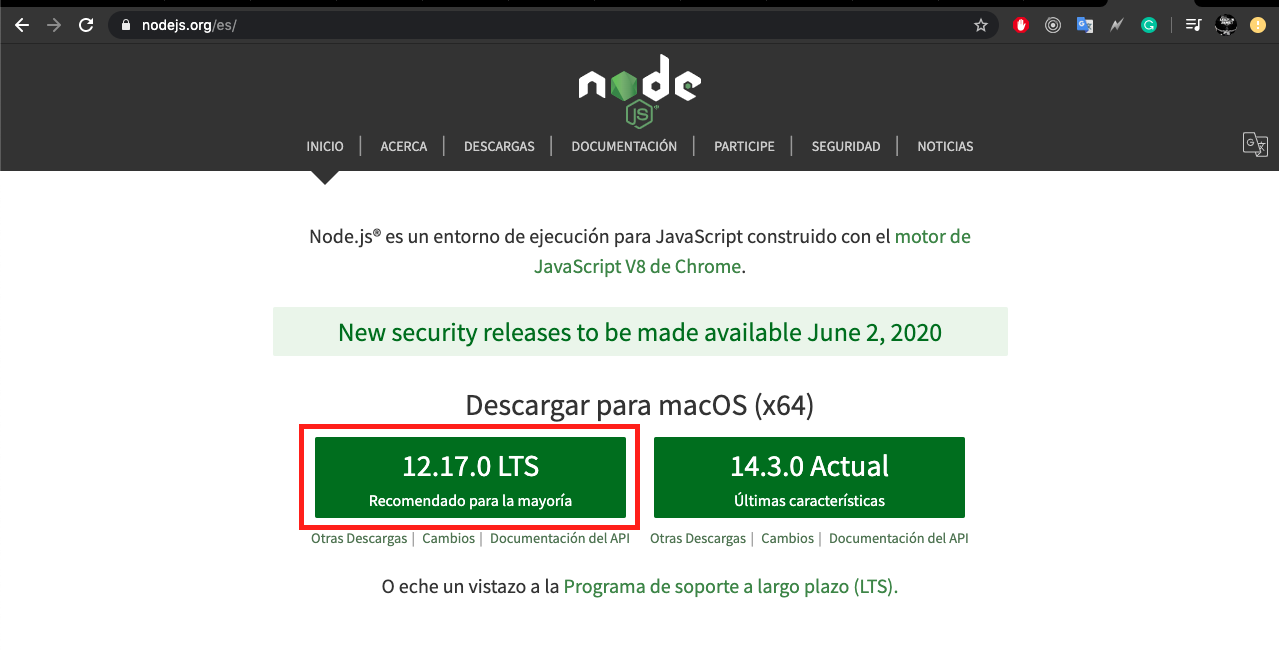
\includegraphics[width = 15cm]{3Proyecto/node}
                \caption{ Descarga de Node JS } 
                \label{fig:node}
           \end{center}
        \end{figure}

        Una vez instalado Node, se abrió una consola de comandos y se ejecutó el comando 'npm install -g @angular/cli' y de esta manera se instaló angular de forma global en el computador.\\

        Para crear el proyecto en Angular se utlizó el comando 'ng new usta-tesis' y de esta forma, Angular generó todos los archivos y dependencias necesarias para generar la aplicación. Una vez hecha la configuración, se derigió a la raiz de proyecto ejecutando el comando 'cd usta-tesis', depués se ejecutó el comando 'ng serve -o' y este comando levanta un servidor local que por defecto es en la dirección http://localhost:4200 y la aplicación ya queda visible para empezar a trabajar en el proyecto. Figura \ref{fig:ngNew}, \ref{fig:ngServe}\\

        \begin{figure}[H]
            \begin{center}
                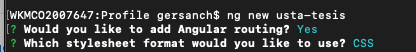
\includegraphics[width = 15cm]{3Proyecto/ngNew}
                \caption{ Creación de proyecto en Angular} 
                \label{fig:ngNew}
           \end{center}
        \end{figure}
        \begin{figure}[H]
            \begin{center}
                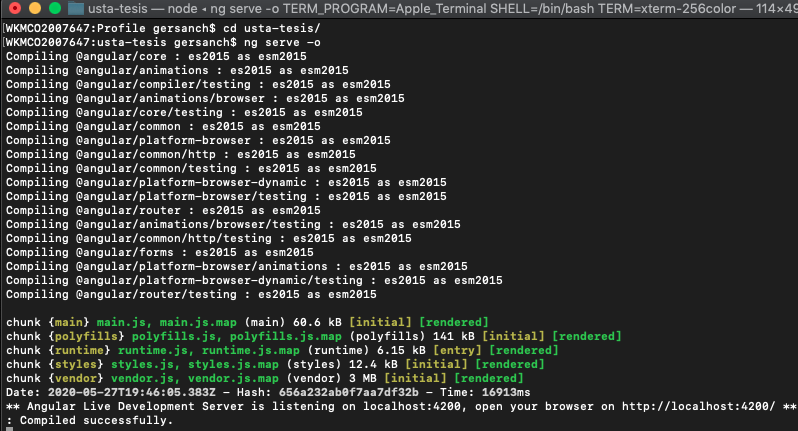
\includegraphics[width = 15cm]{3Proyecto/ngServe}
                \caption{ Levantar servidor local en Angular} 
                \label{fig:ngServe}
           \end{center}
        \end{figure}
        En Angular, un componente hace referencia a una sección visual de la página y estos componentes se crean a través del comando 'ng generate component componentName'. Cada componente cuenta con un archivo .html , .ts y .css. Para el proyectó creamos 4 componentes con los comandos de la figura \ref{fig:ngComponents}.\\
        \begin{figure}[H]
            \begin{center}
                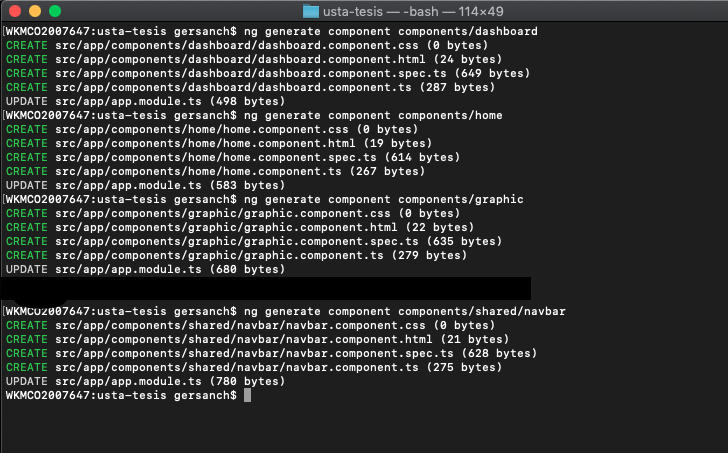
\includegraphics[width = 15cm]{3Proyecto/ngComponents}
                \caption{ Creación de componentes en Angular} 
                \label{fig:ngComponents}
            \end{center}
        \end{figure}

        Con los componentes creados, se empezó a implementar el código necesario para crear la vista, los estilos y la funcionalidad.
        \begin{figure}[H]
            \begin{center}
                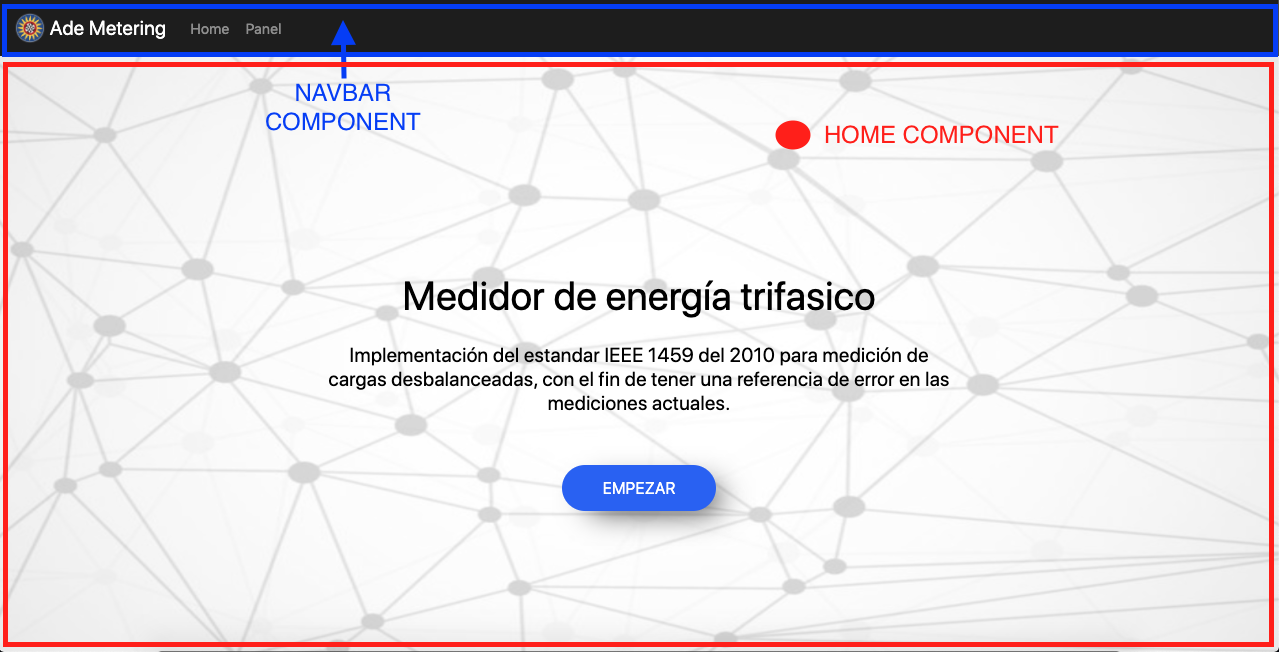
\includegraphics[width = 15cm]{3Proyecto/components1}
                \caption{ Componentes home y navbar} 
                \label{fig:components1}
            \end{center}
        \end{figure}
        \begin{figure}[H]
            \begin{center}
                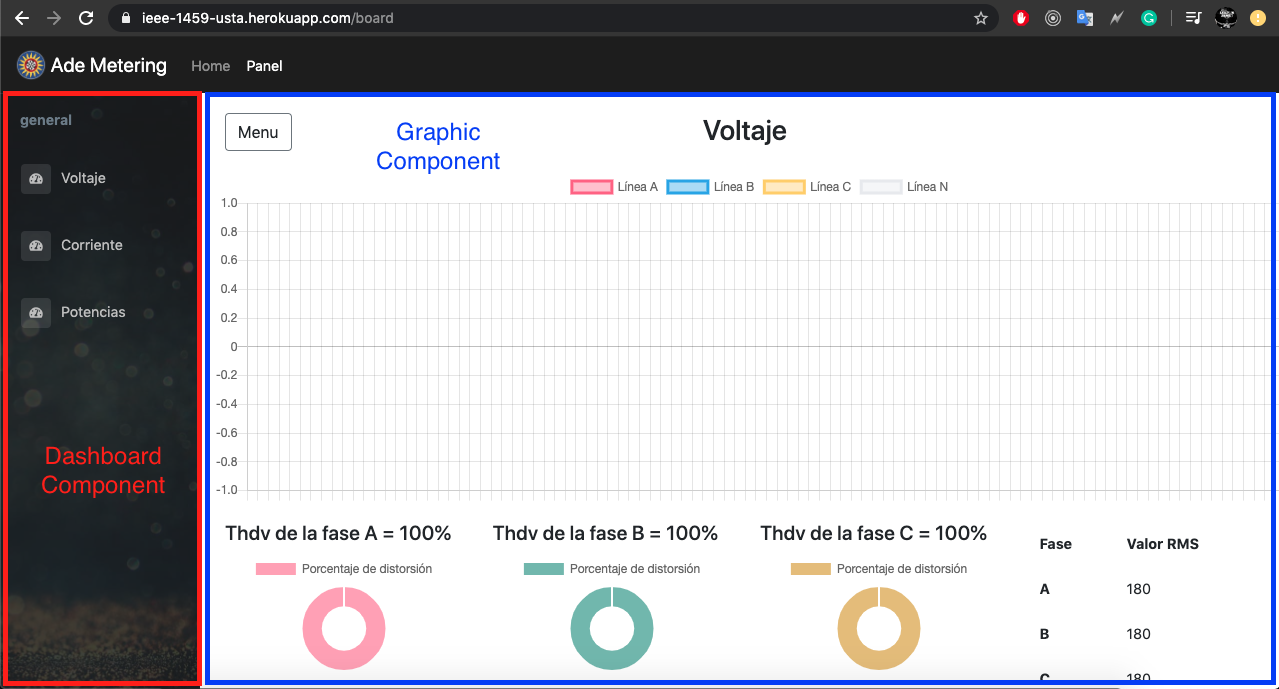
\includegraphics[width = 15cm]{3Proyecto/components2}
                \caption{ Componentes graphic y dashboard} 
                \label{fig:components2}
            \end{center}
        \end{figure}


        \begin{lstlisting}
            
        \end{lstlisting}